\chapter{1994:Avi Wigderson}
\label{chap:wigderson}
\begin{center}
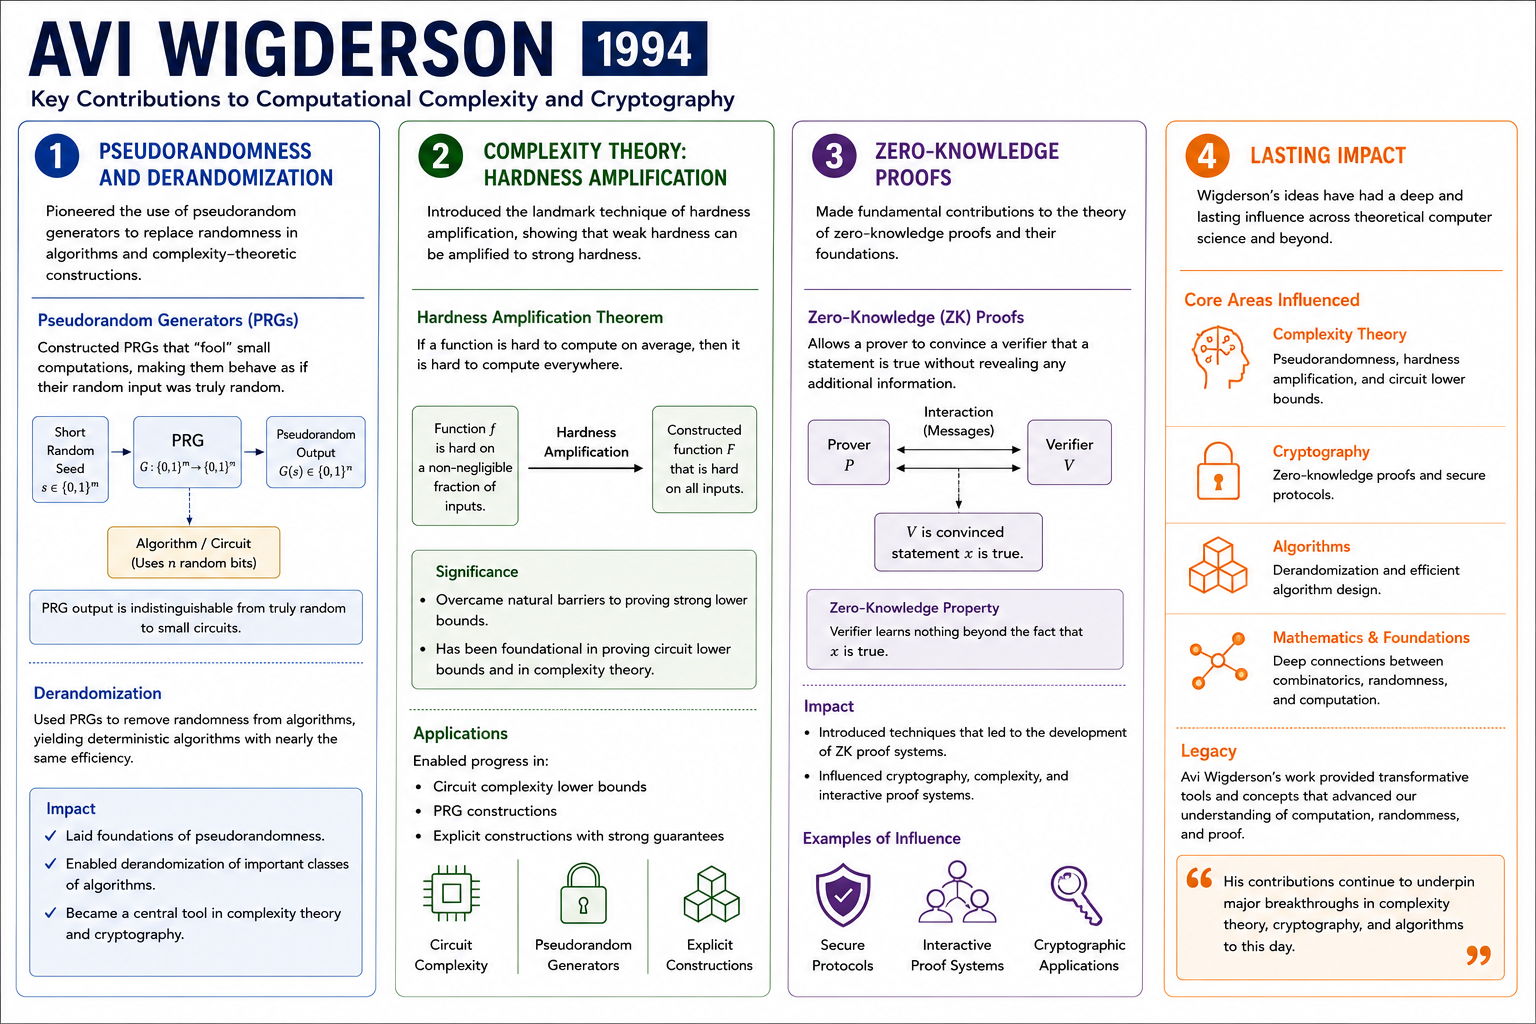
\includegraphics[width=\textwidth]{infographics/abacus4.png}
\end{center}
\targetchapterspacing
\index{Wigderson, Avi}
\booknote{The central habit in this chapter is to let a verifier's random challenge choose what to inspect, and to judge a claimant by the probability of being caught rather than by any single answer.}

\section{An Opening Story: Two Drawings and a Know-It-All}
Two cards lie on a table, each showing a graph on five dots and five lines: one is a five-cycle, the other is a triangle with a two-edge tail attached to one of its vertices. Sam claims he can always tell them apart, even after someone renames the dots.

The teacher tests him. She secretly picks a card, renames all five dots with a fresh shuffle each round, shows the result, and asks: five-cycle or triangle-plus-tail? If the graphs really differ, Sam answers correctly every round. If they secretly showed isomorphic graphs, the rename hides which card was picked and even a perfect answerer is right only half the time; ten rounds of guessing pass with probability $(1/2)^{10}<1/1000$.

Nothing was checked directly. The teacher asked a question she could not answer herself, and the shuffle made it fair: a challenge known in advance could be met with a prepared lie. Randomness turned ``these two are not the same''---a claim with no short written proof---into tests a liar cannot all pass.

\section{The Problem}
One person, the \emph{prover}, claims a fact and will do enormous work to defend it. A second, the \emph{verifier}, has little time and must decide whether to believe it. The prover might lie. How can the verifier be convinced?

The classical answer is a \emph{certificate}: a fixed string a fast deterministic algorithm checks. For ``these two drawings are the same shape'' the certificate is easy: hand over the renaming and compare. The opposite claim, ``these two are \emph{not} the same shape,'' has no known short certificate. For graphs $G_1,G_2$ this is graph non-isomorphism (GNI): an isomorphism witnesses that they \emph{are} the same, but no short static certificate of non-isomorphism is known.

The verifier cannot recompute, cannot trust, and cannot peek inside the prover's head. The escape is conversation: questions the prover could not have anticipated. \emph{Can a weak verifier be convinced of a statement with no short static certificate, by a powerful prover who might be lying?}

\section{The World Before}
For most of the history of logic, a proof was a static object: a certificate string checked mechanically. Computer science inherited this as the class NP: every yes-instance has a short certificate a deterministic verifier accepts, and no no-instance has one. ``Checking is easy, finding is hard'' was the whole vocabulary.

GNI was an embarrassment for that picture. Its no-instances---the isomorphic pairs---have short certificates, namely an isomorphism; its yes-instances have no known short static certificates. Since a certificate can only witness membership, ``not isomorphic'' looked like a problem with no proof at all.

Randomness made things worse before better: randomized algorithms were viewed as a confession of weakness, and the goal was to remove the coin flips. Nobody asked whether a verifier could \emph{use} coin flips as a resource.

What was missing was a proof as a conversation with two extra resources: \emph{interaction} (follow-up questions) and \emph{public randomness} (unpredictable coins). Without both, GNI sat outside any efficient verification framework.

\section{The New Idea}
\subsection{Conversation, not certificate}
An \emph{interactive proof} replaces the certificate with a dialogue. The prover may compute anything; the verifier flips coins, asks questions, and the prover's answer is conditioned on a challenge not known in advance. A pre-announced challenge could be met by one fixed lie; the random challenge is the whole point.

\subsection{The two promises}
\emph{Completeness}: if the claim is true, an honest prover convinces the verifier with high probability. \emph{Soundness}: if it is false, no prover, however clever, convinces it except with small probability. Both probabilities are over the verifier's coins, not the prover's goodwill. Repetition with fresh coins multiplies the error: $1/2$ becomes $(1/2)^k$, below $1/1000$ at $k=10$.

\subsection{Arithmetization: logic becomes algebra}
Rewrite a Boolean computation as polynomial equations over a finite field. A bit $x$ is forced by $x^2-x=0$; AND becomes multiplication ($x\wedge y\mapsto xy$) and OR becomes $x+y-xy$. A circuit becomes one polynomial identity, checked at a few random points.

\subsection{IP = PSPACE}
Lund, Fortnow, Karloff, Nisan, and Shamir proved that every problem solvable with polynomial memory---the class PSPACE---has an interactive proof. A conversation is as powerful as any algorithm for the problem.

\subsection{Zero knowledge: validity without the secret}
Wigderson's signature addition: prove a statement true while revealing nothing about why. A zero-knowledge proof is complete and sound and has transcripts that can be simulated without the witness; if the verifier could have produced the conversation alone, it carries no information. \emph{A proof is not an object; it is a conversation.}

\section{How It Works: Worked Examples}
\subsection{Graph non-isomorphism, round by round}
Let $G_1$ be the five-cycle and $G_2$ the triangle with a two-edge tail attached to one vertex---five vertices and five edges each, not isomorphic. One round: the verifier flips a coin, applies a uniformly random relabeling $\pi$ to the chosen graph, and sends it to the prover, who answers ``five-cycle'' or ``triangle-plus-tail.''

If the claim is true, the honest prover always identifies the graph and passes with probability $1$. If it is false---the graphs \emph{are} isomorphic---a relabeled $G_1$ and a relabeled $G_2$ come from exactly the same distribution, so the answer is independent of the coin and correct with probability $1/2$; ten rounds leave error at most $(1/2)^{10}<1/1000$. The coins matter: a fixed rename could be answered by a memorized lie; a fresh one cannot.

\subsection{Checking a polynomial identity}
The prover claims $x^2=1$ for every $x$. Over $\mathbb{F}_{101}$, the verifier picks a random $r\in\{0,\ldots,100\}$, computes $r^2$ and $1$, and checks equality. The difference $x^2-1=(x-1)(x+1)$ has exactly two roots, $x=1$ and $x=100$, so a random point exposes the lie with probability at most $2/101\approx2\%$. Three independent checks multiply the error to about $(2/101)^3<10^{-5}$.

This is the engine of arithmetization: two distinct polynomials of degree at most $d$ over a field of size $q$ agree at at most $d$ points, so one random evaluation gives meaningful evidence.

\subsection{Zero knowledge on a small graph}
A triangle $a,b,c$ is colored red, blue, red. The prover wants to prove the triangle is $3$-colorable without naming a color. Each round it picks a fresh random permutation of the colors, commits to every vertex's color (hidden until opened), and the verifier picks one of the three edges and asks to open just its two endpoints. The check: the colors differ.

A proper coloring passes every round. A lying prover with a bad edge is caught exactly when that edge is picked, with probability at least $1/3$ per round; $k$ rounds leave error at most $(2/3)^k$, about $1.7\%$ at $k=10$. Nothing leaks because each round uses a fresh permutation: the opened pair is always just ``two distinct colors from three,'' exactly what a simulator without the coloring can reproduce.

\section{The Mathematics in Brief}
An interactive proof for a language $L$ is a pair of machines exchanging messages. For an instance $x$:
\[
x\in L \Rightarrow \PP[V\text{ accepts with honest }P]\geq 2/3,
\qquad
x\notin L \Rightarrow \PP[V\text{ accepts with any }P]\leq 1/3.
\]
The gap between $2/3$ and $1/3$ is deliberate: repetition pushes the $1/3$ toward $0$ exponentially while an honest prover stays accepted. Probabilities are over the verifier's coins only.

The workhorse lemma: \emph{two distinct polynomials of degree at most $d$ over a field of size $q$ agree at at most $d$ points}---their difference is a nonzero polynomial with at most as many roots as its degree.

Arithmetization rests on three exact translations (field of characteristic not $2$):
\[
x\in\{0,1\} \Longleftrightarrow x^2-x=0,\qquad
x\wedge y \Longleftrightarrow xy,\qquad
x\vee y \Longleftrightarrow x+y-xy.
\]
A circuit becomes a system of polynomial equations; a claimed computation becomes a polynomial identity. Lund--Fortnow--Karloff--Nisan and Shamir then proved $\mathrm{IP}=\mathrm{PSPACE}$: interactive proofs capture exactly polynomial memory. Constructively: unwind the computation into a layered circuit, arithmetize it, and verify by a sum-check that justifies a multivariate sum one variable at a time.

Zero knowledge adds a simulation condition: a polynomial-time machine that, given only $x\in L$, produces transcripts indistinguishable from real ones; since it needs no witness, real transcripts cannot be milked for one. The costs are asymmetric: the prover may work exponentially, the verifier polynomially, and soundness error and randomness spent are part of the resource bill.

\section{Limits and Modern Views}
The costs are real: for GNI the prover must actually decide isomorphism, and for arithmetized computations it must manipulate polynomials the verifier never touches. The guarantee is probabilistic, not certain. Zero knowledge adds friction: commitments rest on computational assumptions, transcripts must be rechecked for leakage, and reusing randomness across rounds can destroy privacy.

The ideas outgrew their origin in three directions. \emph{Probabilistically checkable proofs} (PCPs) showed an ordinary NP certificate can be checked by reading a handful of bits---a static object with interactive power. \emph{Succinct proofs} (SNARKs, STARKs) let a cloud computer convince a laptop that a huge computation ran correctly, trading prover time against tiny proofs, amid debates about trusted setup and proof length. \emph{Post-quantum cryptography} asks whether the assumptions behind commitments and succinct proofs survive a quantum adversary, and answers with lattice problems \cite{wigderson-interactive,wigderson-zk}. The lessons persist: expose algebraic structure, sample random constraints instead of rechecking everything, and separate validity from secrecy.

\section{Exercises and Self-Study Guide}
\begin{enumerate}[label=\textbf{E\arabic*.}]
\item Write the polynomial constraint that forces a variable to be a bit, and verify it in $\mathbb{F}_3$ at $x=0,1,2$.
\hint{$x^2-x=0$; $x=2$ gives $4-2=2\neq0$, and note why the trick silently fails in $\mathbb{F}_2$.}
\item Show that $P(x)=x^2$ and $Q(x)=1$ agree at exactly two points in $\mathbb{F}_7$, and list them.
\hint{Solve $x^2=1$ over $\{0,\ldots,6\}$; the solutions are $x=1$ and $x=6$, so a random point catches the difference with probability $5/7$.}
\item A protocol has soundness error $1/3$. Find the smallest $k$ such that $k$ independent rounds bring the error below $1/100$.
\hint{$(1/3)^4=1/81$ is still above $1/100$; $k=5$ gives $1/243$.}
\item Construct a zero-knowledge transcript that accidentally reveals the witness, using the $3$-coloring protocol on the triangle.
\hint{Reuse the same color permutation in two rounds opening two edges that share a vertex; combining the opened colors pins down the full coloring.}
\item Compute the soundness error of the GNI protocol for $k=5$ rounds, and state the honest prover's acceptance probability.
\hint{$(1/2)^5=1/32\approx3\%$; the honest prover is still accepted with probability $1$.}
\item Convert the Boolean formula $(x\wedge y)\vee z$ into polynomial equations, including bit constraints.
\hint{Introduce $a=xy$ for the AND; the OR becomes $a+z-az$; each variable satisfies $t^2-t=0$.}
\item Explain why the verifier must not reveal its random challenge before the prover answers, using GNI.
\hint{A pre-announced rename is a single test with a memorized answer; randomness makes every round a fresh test.}
\end{enumerate}

\booknote{A final exercise in judgment: before trusting any verification system, name what the verifier's random coins protect against. If the answer is ``a prepared lie,'' find the challenge the prover cannot predict; if you cannot name it, the protocol is only a certificate wearing a costume.}
\clearpage
